% !TEX encoding = UTF-8 Unicode
%%% Template originaly created by Karol Kozioł (mail@karol-koziol.net) and modified for ShareLaTeX use
\documentclass[a4paper,11pt]{article}
\usepackage[french]{babel} % English language/hyphenation
\usepackage{mathptmx} % Use the Adobe Times Roman as the default text font together with math symbols from the Sym­bol, Chancery and Com­puter Modern fonts

\usepackage[T1]{fontenc}
\usepackage{ucs}
\usepackage[utf8x]{inputenc}
\usepackage{lipsum} % Inserts dummy text
\usepackage{graphicx}
\usepackage{color}

\renewcommand\familydefault{\sfdefault}
\usepackage{tgheros}
%\usepackage[defaultmono]{droidmono}

\usepackage{amsmath,amsfonts,amssymb,amsthm} % For math equations, theorems, symbols, etc
\usepackage{enumerate}
\usepackage{multicol}
\usepackage{tikz}
\usepackage[tikz]{bclogo}
\usepackage{multicol}
\usepackage{geometry}
\geometry{total={210mm,297mm},
left=25mm,right=25mm,%
bindingoffset=0mm, top=20mm,bottom=20mm}
\usepackage{url}
\usepackage[linkbordercolor=blue]{hyperref}
\author{M. A. Ammar - IPEST : HAP}
\date{16 décembre 2020}
\setlength{\parindent}{0pt}



\linespread{1.3}

\newcommand{\linia}{\rule{\linewidth}{0.5pt}}

% custom theorems if needed
\newtheoremstyle{mytheor}
    {1ex}{1ex}{\normalfont}{0pt}{\scshape}{.}{1ex}
    {{\thmname{#1 }}{\thmnumber{#2}}{\thmnote{ (#3)}}}

\theoremstyle{mytheor}
\newtheorem{defi}{Definition}

% my own titles
\makeatletter
\renewcommand{\maketitle}{
\begin{center}
\vspace{2ex}
{\huge \textsc{\@title}}
\vspace{1ex}
\\
\linia\\
\@author \hfill \@date
\vspace{4ex}
\end{center}
}
\makeatother
%%%

% custom footers and headers
\usepackage{fancyhdr}
\pagestyle{fancy}
\lhead{}
\chead{}
\rhead{}
\lfoot{}
\cfoot{}
\rfoot{Page \thepage}
\renewcommand{\headrulewidth}{0pt}
\renewcommand{\footrulewidth}{0pt}

%%%%%%%%%%%%%%%%%%%%%%%%%%%%%%%%%%%%%%%%
%%%%%%%%%%%%%%%%%%%%%%%%%%%%%%%%%%%%%%%%%
%%%% CODE
%%%%%%%%%%%%%%%%%%%%%%%%%%%%%%%%%%%%%%%%
\usepackage{fancyvrb} % packages needed for verbatim environments
\usepackage{listingsutf8}

\definecolor{mygreen}{rgb}{0,0.6,0}
\definecolor{mygray}{rgb}{0.5,0.5,0.5}
\definecolor{mymauve}{rgb}{0.58,0,0.82}
\DeclareFixedFont{\ttb}{T1}{pcr}{bx}{n}{10} % for bold
\DeclareFixedFont{\ttm}{T1}{pcr}{m}{n}{10}  % for normal
\lstset{ 
	backgroundcolor=\color{lightgray!10},   % choose the background color; you must add \usepackage{color} or \usepackage{xcolor}; should come as last argument
	basicstyle=\ttm,        % the size of the fonts that are used for the code
	breakatwhitespace=false,         % sets if automatic breaks should only happen at whitespace
	breaklines=true,                 % sets automatic line breaking
	postbreak=\raisebox{0ex}[0ex][0ex]{\ensuremath{\color{red}\hookrightarrow\space}},
	captionpos=b,                    % sets the caption-position to bottom
	commentstyle=\color{mygreen},    % comment style
	deletekeywords={...},            % if you want to delete keywords from the given language
	escapeinside={\%*}{*)},          % if you want to add LaTeX within your code
	extendedchars=true,              % lets you use non-ASCII characters; for 8-bits encodings only, does not work with UTF-8
	firstnumber=1,                % start line enumeration with line 1000
	frameround=fttt,
	frame=single,	                   % adds a frame around the code
	keepspaces=true,                 % keeps spaces in text, useful for keeping indentation of code (possibly needs columns=flexible)
	keywordstyle=\ttb\color{blue},       % keyword style
	language=Python,                 % the language of the code
	morekeywords={*,...},            % if you want to add more keywords to the set
	numbers=left,                    % where to put the line-numbers; possible values are (none, left, right)
	numbersep=5pt,                   % how far the line-numbers are from the code
	numberstyle=\tiny\color{mygray}, % the style that is used for the line-numbers
	rulecolor=\color{black},         % if not set, the frame-color may be changed on line-breaks within not-black text (e.g. comments (green here))
	showspaces=false,                % show spaces everywhere adding particular underscores; it overrides 'showstringspaces'
	showstringspaces=false,          % underline spaces within strings only
	showtabs=false,                  % show tabs within strings adding particular underscores
	stepnumber=1,                    % the step between two line-numbers. If it's 1, each line will be numbered
	stringstyle=\color{mymauve},     % string literal style
	tabsize=4,	                   % sets default tabsize to 2 spaces
	title=\lstname                   % show the filename of files included with \lstinputlisting; also try caption instead of title
}
\usepackage{textcomp}
\DefineVerbatimEnvironment % create new one
{pyshell}{Verbatim}{frame=leftline, framerule=1.5mm, rulecolor=\color{blue}}
\begin{document}
	
\title{Épreuve d'informatique (Python) \textnumero 1 \\ (corrigé)}

\maketitle

\section*{Exercice 1 : Calculer les niveaux d'énergie dans un atome}
Le $n^{ième}$ niveau d'énergie d'un électron dans un atome d'hydrogène est donné par:
\begin{equation}
E_n = -\frac{m_e e^4}{8\epsilon_0^2h^2}\cdot\frac{1}{n^2} ,
\end{equation}
où $m_e = 9.1094⋅10^{-31} \ kg$ est la masse de l'électron, $e = 1.602210^{−19} \ C$ est la charge élémentaire, $\epsilon_0 = 8.8542 \cdot 10^{-12} C^2 s^2 \ kg^{-1}m^{-3}$ est la permittivité électrique du vide, et $h=6.6261 \cdot 10^{−34} \ Js$


\begin{itemize}
\item[\textbf{Q1.}] On défini d'abord les constantes dans l'équation, ensuite la fonction \texttt{E(n)} qui retourne la valeur du niveau d’énergie en électron-volt ($eV$):
\begin{lstlisting}
# Constantes
me = 9.1094e-31
e = 1.6022e-19
eps0 = 8.8542e-12
h = 6.6261e-34
def E(n):
    Ejoule = - (me * e**4)/(8*eps0**2 * h**2)* (1/n**2)
    return Ejoule/e
\end{lstlisting}


\item[\textbf{Q2.}] Le niveau d'énergie pour n = 1:
\begin{lstlisting}
print("E(n = 1) = ", E(n = 1), " eV")
# ==> E(n = 1) =  -13.606152702370753  eV
\end{lstlisting}
\noindent
Le niveau d'énergie le plus bas $E_1 = - 13,6 \ eV$ obtenu pour n = 1, correspond au niveau fondamental de l'atome d'hydrogène. C'est l'état le plus stable.

\item[\textbf{Q3.}] Le niveau d'énergie pour n = 100:
\begin{lstlisting}
print("E(n = 100) = ", E(n = 100), " eV")
# ==> E(n = 100) =  -0.0013606152702370755  eV
\end{lstlisting}
Le niveau d'énergie est nul $E = 0 \ eV$  lorsque n tend vers l'infini (l'électron est alors séparé du noyau).

\item[\textbf{Q4.}] On peut calculer et afficher les valeurs $E_n$ pour $n = 1,…, 20$ en utilisant une boucle for:
\begin{lstlisting}
for n in range(1, 21):
    print("E{} = {} eV".format(n, E(n)))
\end{lstlisting}
Le résultat doit être comme suivant:
\begin{pyshell}
E1 = -13.606152702370753 eV
E2 = -3.4015381755926883 eV
............................
............................
E19 = -0.03769017369077771 eV
E20 = -0.03401538175592689 eV
\end{pyshell}
\item[\textbf{Q5.}] On peut créer la matrice $\Delta E^{i,f}$ et afficher ces valeurs avec la méthode suivante:

\begin{lstlisting}
from numpy import array
DEn = [[E(ni) - E(nf) for ni in range(1, 6)] for nf in range(1,6)]
print(array(DEn))
#==> DEn =
#[[  0.          10.20461453  12.09435796  12.75576816  13.06190659]
# [-10.20461453   0.           1.88974343   2.55115363   2.85729207]
# [-12.09435796  -1.88974343   0.           0.6614102    0.96754864]
# [-12.75576816  -2.55115363  -0.6614102    0.           0.30613844]
# [-13.06190659  -2.85729207  -0.96754864  -0.30613844   0.        ]]
\end{lstlisting}
\end{itemize}
\section*{Exercice 2 : Tracer la viscosité de l'eau}
La viscosité de l'eau, $\mu$, varie avec la température $T$ (en Kelvin) selon la formule:
\begin{equation}
\mu (T) = A\cdot 10^{B/(T-C)}
\end{equation}
où $A=2.414\cdot 10^{-5}\hbox{ Pa s}$, $B=247.8 \ K$ et $C = 140 \ K$.


\begin{itemize}
\item[\textbf{Q1.}] La fonction \texttt{mu(T, A, B, C)} est définie comme suivant:
\begin{lstlisting}
def mu(T, A, B, C):
    return A*10**(B/(T-C))
\end{lstlisting}
\newpage
\item[\textbf{Q2.}] Le code qui trace la viscosité de l'eau en fonction de la température est comme suivant:
\begin{lstlisting}
import matplotlib.pyplot as plt
import numpy as np
# 0 deg C = 273 deg K
T = np.linspace(0, 100, 20)

plt.plot(T, mu(T+273, A = 2.414e-5, B = 247.8, C = 140), 'k^--')
plt.title("Évolution de la viscosité de l'eau avec la température",
          fontweight='bold')
plt.xlabel("Température (degrés Celsius)")
plt.ylabel("Viscosité (Pa s)")
plt.grid()
\end{lstlisting}
\end{itemize}
% --- begin hint in exercise ---

\begin{bclogo}[logo=\bclampe, couleurBarre=green, noborder=true, couleur=yellow!10]{Indications.}
\begin{itemize}
\item On vous rappelle que : 0 $^\circ$C = 273 $^\circ$K.
\item La sortie du programme devrait ressembler à la figure ci-dessous.

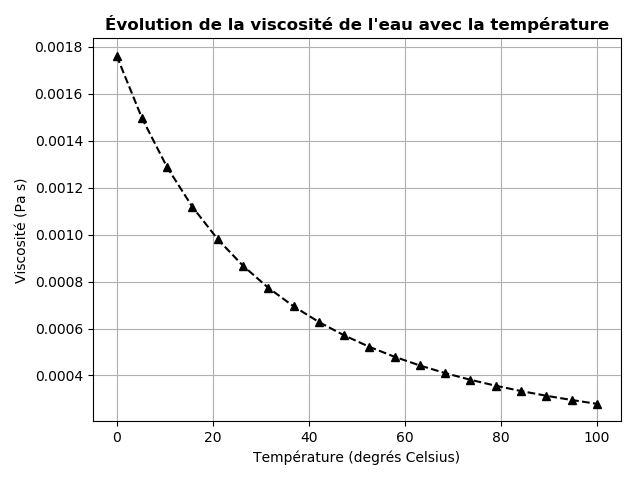
\includegraphics[width=0.7\linewidth]{figures/viscosity}
\end{itemize}
\end{bclogo}
\section*{Exercice 3 : Diffraction par ouverture rectangulaire}
Considérons un faisceau de lumière monochromatique de longueur d'onde $\lambda$ éclairant une ouverture rectangulaire située dans un plan $(xOy)$. La largeur de l'ouverture $b$ est dans la direction $x$ et sa hauteur $h$ est dans la direction $y$.

L'intensité normalisée de lumière en un point $M$ situé sur un écran ($E$) et à une distance $D$ de la fente peut s'écrire comme suit :
\begin{equation}
\dfrac{I(x_{M}, y_{M})}{I_{0}} = \text{sinc}^{2}\left (B \cdot x_{M} \right)\,\text{sinc}^{2}  \left ( H \cdot y_{M} \right )
\label{Eq_1_3}
\end{equation}
%
où $H = \frac{\pi h}{\lambda D}$, $B = \frac{\pi b}{\lambda D}$.

\begin{itemize}
\item La largeur de la tache centrale dans la direction $x$ est inversement proportionnelle à la largeur de l'ouverture: $\Delta x = \frac{2 \lambda D}{b}$;
\item La largeur de la tache centrale dans la direction $y$ est inversement proportionnelle à la hauteur de l'ouverture : $\Delta y = \frac{2 \lambda D}{h}$.
\end{itemize}

La fonction Python \verb|DiffRect(lamda, b, h, D)|, qui calcul $\Delta x$ et $\Delta y$ et affiche la figure de diffraction, peut s'écrire comme suivant :
\lstinputlisting{scripts/DiffRect.py}
\newpage
\begin{pyshell}
>>> DiffRect(lamda= 630*1.E-9, b= 2*1.E-5, h= 4*1.E-5, D= 2)
La largeur de la tache centrale dans la direction x :  12.6
La largeur de la tache centrale dans la direction y :  6.3
\end{pyshell}
\begin{figure*}[th!]
\centering
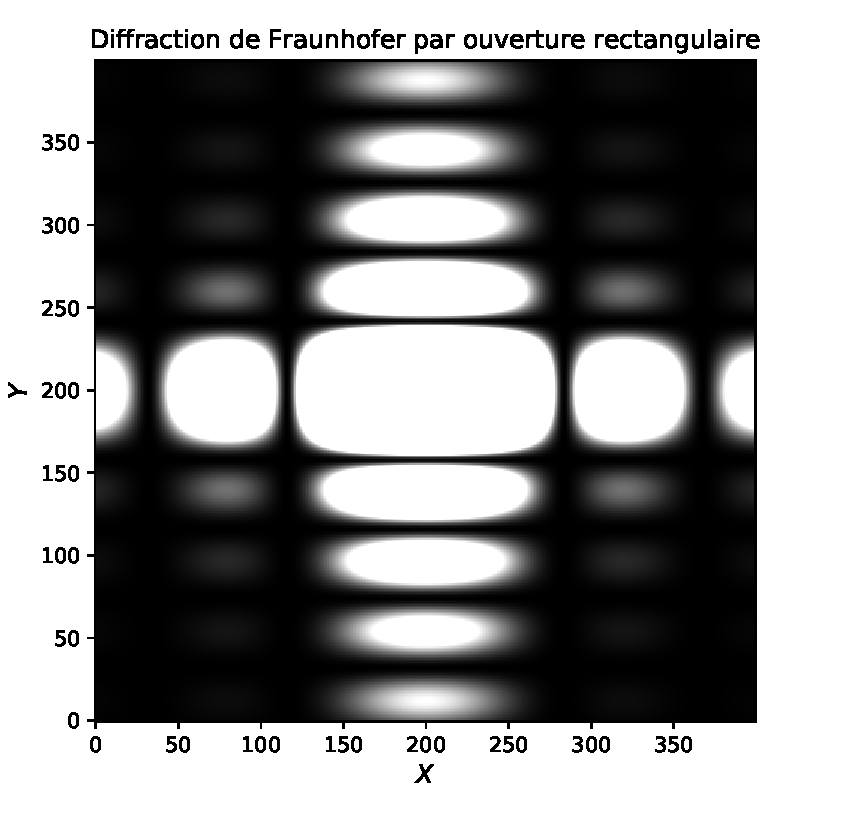
\includegraphics[width=0.7\linewidth]{figures/figureDiff}
\end{figure*}

\end{document}
